To examine whether the calibration and simulation results transferred to later observations, we extended the evaluation beyond the original April--May window. The completed expanding-window experiment evaluated two-input sector networks on 53 successive held-out capture dates through July 17. Median test RMSE was 9.92 IV percentage points, but individual folds ranged from 7.68 to 19.25 points (Supplementary Table~\ref{tab:walk_forward_extended}). This spread showed that the pooled surface representation transferred unevenly across dates. Each fold used the later observation's stock price to determine moneyness, so the result concerned conditional IV prediction rather than a forecast of the stock--option system. We then fitted a single set of sector surfaces through July 31 and evaluated the 23 later sessions from August 4 through September 4. Pooled RMSE increased from 10.79 points in training to 14.75 points in the held-out sample (Supplementary Table~\ref{tab:chronological_surface}). These values were not a paired comparison with the earlier folds because the fitting window, capture audit, and evaluation dates differed. The GS surface had held-out RMSE of 6.30 points and mean overprediction of 0.88 points, whereas LLY had RMSE of 9.96 points and mean overprediction of 4.61 points. The larger corpus therefore did not remove the problem of a frozen surface level lagging a later market state. This motivated a separate forecast comparison in which all IV variants started from the observed origin IV and differed in their subsequent evolution (Section~\ref{sec:chronological_methods}).

The forward evaluation compared forecasts with later observations of the same selected contracts. The maturity-bucket collection scheme imposed an immediate limit: none of the 36 eligible roughly monthly contracts per ticker had an observed exact-symbol endpoint after five sessions (Supplementary Table~\ref{tab:forecast_availability}). Their one-session comparison retained 34 quotes across 17 origins per ticker. Coupled-factor MAE was \$3.79 per share for GS and \$6.08 for LLY, compared with \$3.80 and \$6.11 under frozen IV (Supplementary Table~\ref{tab:forecast_one_session}). The separately identified shorter-maturity cohort supplied five-session outcomes for 34 GS and 30 LLY quotes across 17 origins per ticker. Coupling again produced only small reductions in absolute error of the forecast mean: MAE was \$4.19 versus \$4.21 under frozen IV for GS, and \$11.59 versus \$11.62 for LLY (Table~\ref{tab:forecast_main}). It improved the date-level mean absolute error on six of seventeen GS origins and nine of seventeen LLY origins, so the small average reductions did not show a consistent advantage across dates. Scoring forecast medians separately lowered GS coupled-factor MAE to \$2.48 and gave LLY MAE of \$11.79, with little separation from frozen IV (Supplementary Table~\ref{tab:option_point_summary}). The coupled model's CRPS was 2.01 for GS and 8.93 for LLY, compared with 2.02 and 8.99 under frozen IV. Central 90\% intervals had date-weighted coverage of 100\% for GS and 67.6\% for LLY, with average widths of \$25.65 and \$28.91 per share. Broad coverage in GS therefore coexisted with substantial missed coverage in LLY. The earliest eligible GS example showed nearly coincident coupled and frozen-IV mean forecasts while the observed call value declined below both means (Fig.~\ref{fig:chronological_forecast}). These results supported a limited chronological case study of the assembled model, but they did not establish a material forecasting advantage from the fixed stochastic factor or validate the original month-long illustrations.

\begin{table}[H]
\centering
\caption{Five-session option forecasts for the shorter-maturity cohort, selected with 10--21 calendar DTE at each origin. Scores average matched contracts within each ticker and origin before averaging dates. MAE scores the forecast mean; MAE, CRPS, and central 90\% interval width are dollars per share. Coverage is date-weighted. Every IV variant uses the same stock paths, origin IV, and matched quotes.}\label{tab:forecast_main}
\resizebox{\textwidth}{!}{\begin{tabular}{llrrrrrr}
\toprule
Ticker & IV variant & Dates & Quotes & MAE & CRPS & Coverage (\%) & Width \\
\midrule
GS & Frozen IV & 17 & 34 & 4.21 & 2.02 & 100.0 & 25.64 \\
GS & Direct surface & 17 & 34 & 4.86 & 2.16 & 67.6 & 24.01 \\
GS & Mean reversion & 17 & 34 & 4.26 & 2.02 & 100.0 & 25.62 \\
GS & Uncoupled factor & 17 & 34 & 4.24 & 2.03 & 100.0 & 25.69 \\
GS & Coupled factor & 17 & 34 & 4.19 & 2.01 & 100.0 & 25.65 \\
LLY & Frozen IV & 17 & 30 & 11.62 & 8.99 & 73.5 & 28.98 \\
LLY & Direct surface & 17 & 30 & 11.62 & 9.05 & 55.9 & 26.68 \\
LLY & Mean reversion & 17 & 30 & 11.62 & 8.99 & 73.5 & 28.83 \\
LLY & Uncoupled factor & 17 & 30 & 11.61 & 8.97 & 73.5 & 28.83 \\
LLY & Coupled factor & 17 & 30 & 11.59 & 8.93 & 67.6 & 28.91 \\
\bottomrule\end{tabular}
}
\end{table}

\begin{figure}[H]
\centering
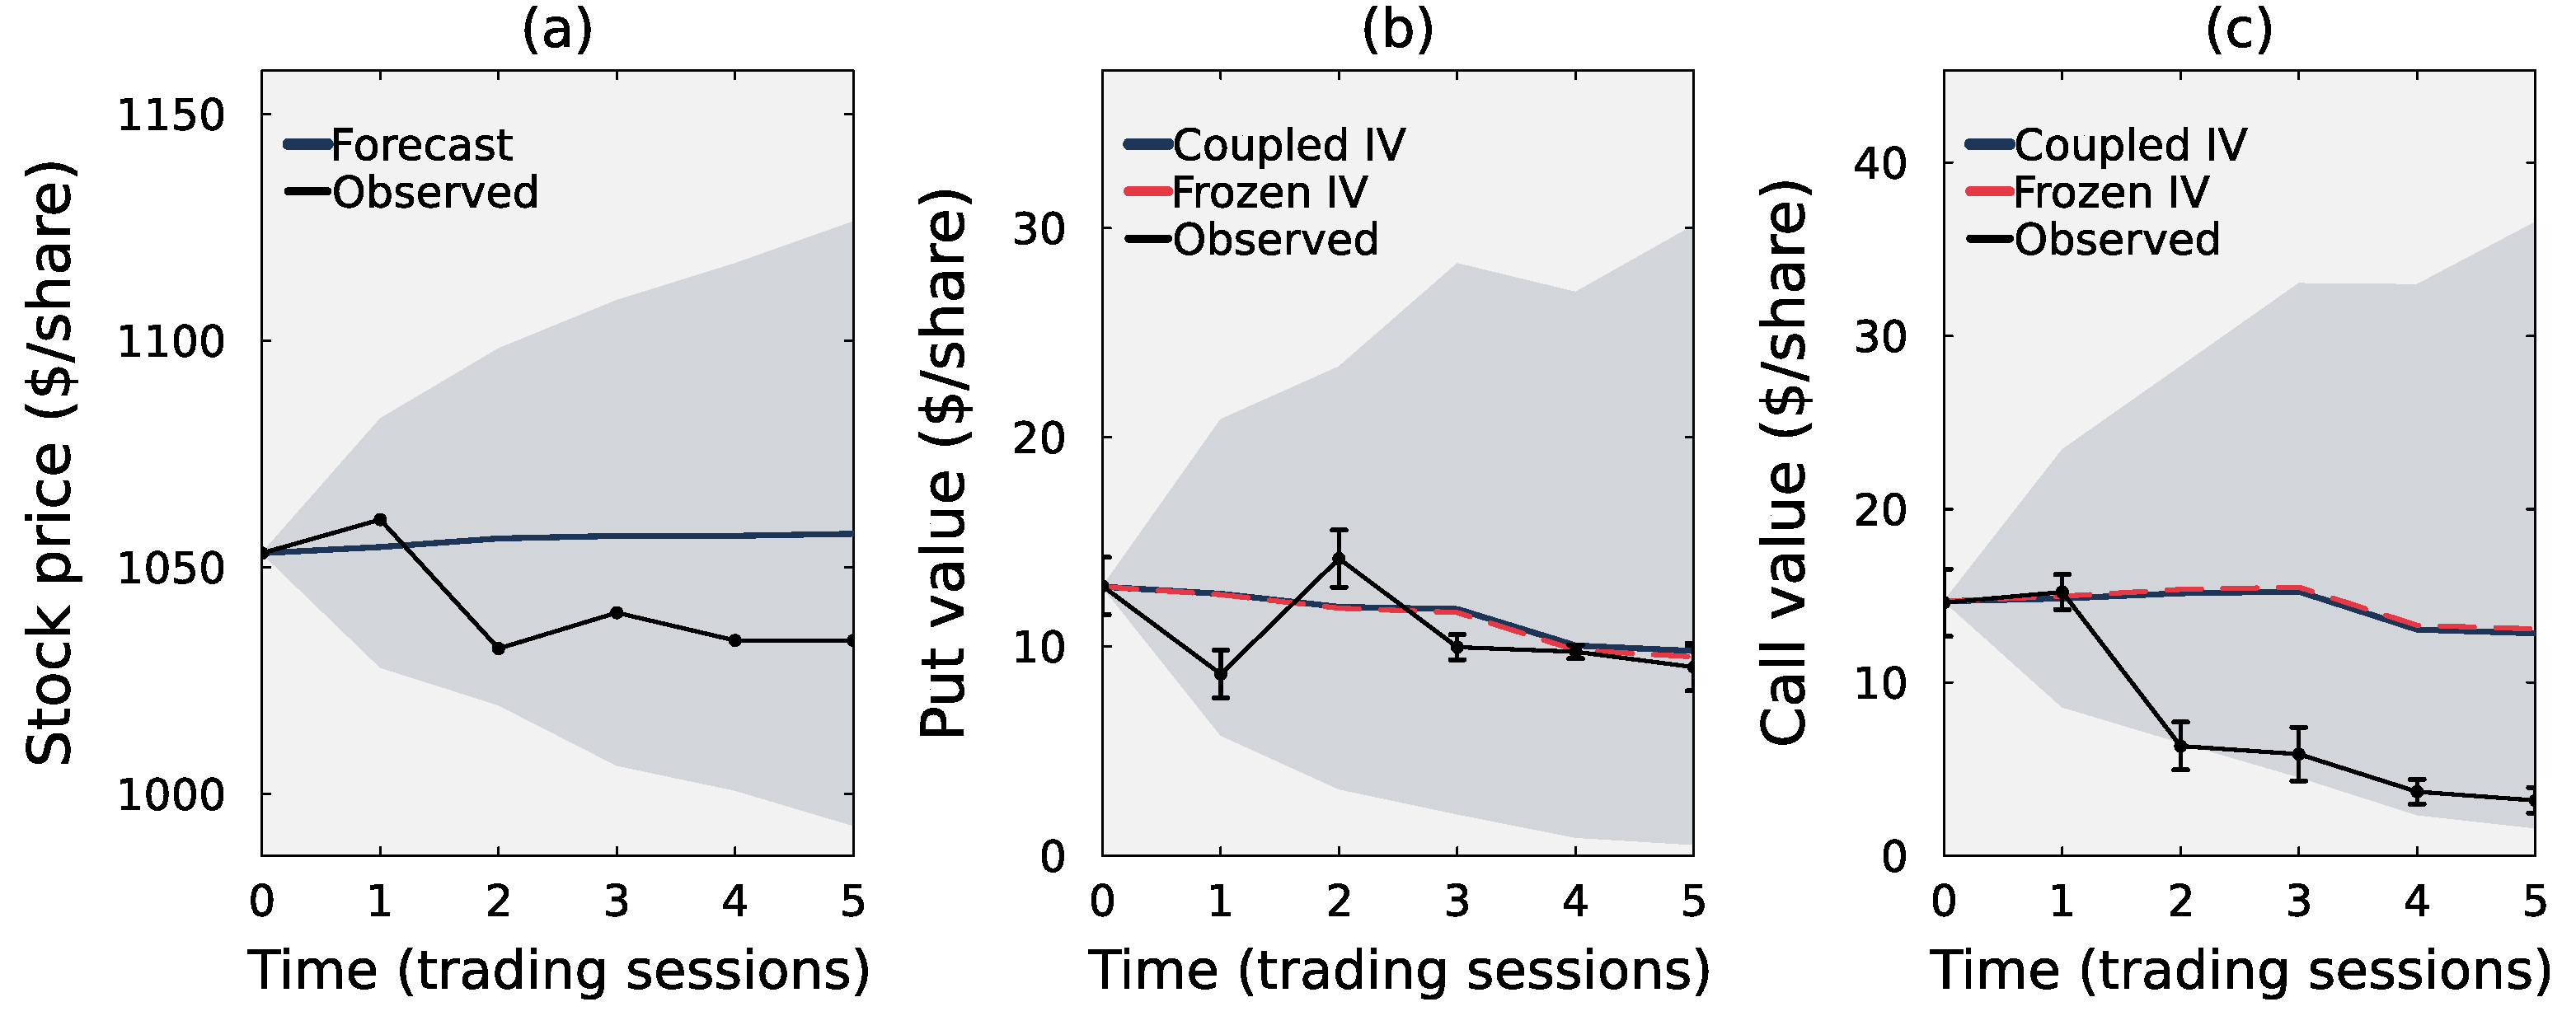
\includegraphics[width=\textwidth]{sections/figures/chronological_forecast.pdf}
\caption{Five-session forecasts of GS stock prices (a), put values (b), and call values (c), compared with observations from August 4 to August 11, 2026. The put strike is \$1{,}000, the call strike is \$1{,}105, and both contracts expire on August 21. Forecasts use the July-cutoff surface and information available at the August 4 origin. Navy curves show forecast means from 1{,}000 stock paths, with the coupled IV factor used for option values; shading spans the central 90\% of simulated values. Red dashed curves show frozen-IV mean option forecasts on the same stock paths. Black points show observed stock closes and option midpoints, with vertical bars spanning Alpaca's indicative bid and ask. These option observations are vendor values rather than exchange quotes. Time is measured in exchange sessions from the origin. This is the earliest GS origin with both selected shorter-maturity contracts observed at the five-session endpoint.}\label{fig:chronological_forecast}
\end{figure}

We used the observed-stock diagnostic to distinguish stock-path errors from the IV and pricing components on a common subset. Complete intervening stock observations were available for thirteen five-session origins per ticker, with 26 matched GS quotes and 24 LLY quotes. On these same cases, replacing simulated stock paths with the observed path reduced coupled-factor MAE from \$4.62 to \$1.23 per share for GS and from \$10.61 to \$1.95 for LLY. The observed path was supplied after the forecast period and would have been unknown at the origin. This calculation diagnosed error sources; it was not an attainable improvement to the forward forecast. Within that diagnostic, frozen IV had lower point errors of \$1.07 and \$1.74, while uncoupled stochastic factors had lower CRPS than the coupled factor for both tickers (Supplementary Table~\ref{tab:forecast_conditional}). The stock comparison also gave no point-forecast advantage to the retained JumpHMM settings: five-session stock MAE was \$16.85 for GS and \$49.83 for LLY, versus \$16.17 and \$48.64 for the simple random walk (Supplementary Table~\ref{tab:forecast_stock}). Repricing the shorter-maturity endpoint observations with their reported IV reduced five-session option MAE to \$0.14 for GS and \$0.34 for LLY, and those prices lay within every observed bid--ask interval (Supplementary Table~\ref{tab:forecast_repricing}). Sampled lattice refinement changed marks by at most \$0.0026 per share across the two cohorts, well below the forecast errors. Together, these diagnostics showed that stock-forecast errors contributed substantially to the option-price misses, with additional error remaining in the IV and pricing inputs. They did not establish why the stock estimator missed or how to correct it. They did not identify a reliably superior dynamic variant. The small, overlapping set of origins, missing contract histories, fixed parameters, and absence of quote-level exchange timestamps limited broader conclusions about forecasting accuracy or executable trading performance.
The wider return-cutoff comparison repeated the same chronological forecasts and stock benchmarks. Widening the residual bound from $b=10$ to $b=20$ changed five-session coupled option MAE by less than \$0.007 per share and the reported stock CRPS values by less than \$0.002 (Supplementary Table~\ref{tab:tail_forecasts}). These changes did not alter the conclusions of the specified forecast comparisons.
\FloatBarrier
